\documentclass[14pt,a4paper]{article}
\usepackage[utf8]{inputenc}
\usepackage{amsmath}
\usepackage{amsfonts}
\usepackage{amssymb}
\usepackage{graphicx}
\usepackage[left=2cm,right=2cm,top=2cm,bottom=2cm]{geometry}
\usepackage[
    backend=bibtex,
    %style=alphabetic,
    sorting=ynt
]{biblatex}
\addbibresource{../biblio.bib}
\usepackage{hyperref}
\hypersetup{
    colorlinks=true,
    linkcolor=cyan!60!white,
    filecolor=magenta,
    urlcolor=cyan,
    pdftitle={Sharelatex Example},
    bookmarks=true,
    pdfpagemode=FullScreen,
}
\usepackage{float}
\floatplacement{figure}{H}
\usepackage{caption}
\usepackage{subcaption}
%\usepackage{subfig}

%------------%
% Author Info
%------------%
\author{
  \hspace*{1.5em} Soham Naha\\
  \hspace*{1.5em} \texttt{193079003}
  \and
  Mohit Agarwala\\
  \texttt{19307R004}
  \and
  Abhinav Goud Bingi\\
  \texttt{180050002}\\[1.5cm]
}
%------------%
% Title Info
%------------%
\title{\textsc{\LARGE Indian Institute of Technology}\\[1.5cm] % Name of your university/college
\begin{center}

\includegraphics[height=6cm,width=6cm]{../images/iitb_logo.png}
\end{center}
\textsc{\Large CS 753 Project Report}\\[0.5cm]
\HRule \\[0.4cm]
{ \huge \bfseries Speech to Sign-Language(with emotions) for the Hearing-Impaired}\\[0.4cm] % Title of your document
\HRule \\[1.5cm]
\textbf{Reported By}}
%------------%
% Date Info
%------------%
\date{{\large \today}\\[2cm]}
\newcommand{\HRule}{\rule{\linewidth}{0.5mm}}


\begin{document}
\maketitle

\newpage
\section{Problem Statement and Motivation}
A speech and/or hearing impaired person communicates with others using Sign-Language (SL), that is different from the speech modes of communication. There are a lot of literatures that deal with the problem of conversion from Sign-Language (predominantly American Sign Language or ASL) letters to speech, but the reverse domain is not much explored.

\subsection{Problem Statement}
We choose to explore the domain from speech to ASL. So, our primary task was, given a speech utterence from a speaker convey a message to a person who is hearing-impaired and/or voiceless, then speech has to be converted in a form that the other person can understand, i.e. in a sign language.

\subsection{Motivation}
Most of the literature that is present regarding the field of SL and Speech are related to the field of SL-to-Speech conversion with limited vocabulary datasets.

But research related to the other direction, i.e. from Speech-to-SL is not much explored. In this project, we thus aimed to explore the domain from Speech to Sign-Language with the help of Automatic Speech Recognition. 
This could be used as a conversation model for the speech and/or hearing impaired to interact freely with people who don't have knowledge of SL.

It is also noticeable that conversion of speech-to-SL does not necessarily contain the emotion conveyed through the utterence. So, we also tried to add this emotion part along with the other decodings.


\section{Task at Hand}
In order to convert from Speech-to-SL along with emotions, we tried to follow the approach as stated below:
\begin{itemize}
	\item Convert Speech to English Text
	\item Guess the Emotion conveyed within the utterence in parallel to text estimation
	\item Use the predicted text to estimate the sign-language patterns.
\end{itemize}
So, we modularized the complete pipeline into different blocks that can be trained and modelled independently and integrated again. The modules that we have are thus:
\begin{itemize}
	\item Speech2text
	\item Emotion Detection from Audio
	\item Text2ASL
\end{itemize}
Now we look into each of these individual modules sequentially. 

\subsection{Speech2Text}
A large part of Automatic Speech Recognition (ASR) is dedicated to the task of conversion of Speech to Text. This conversion can predict as output entire word ( or grapheme) sequences, or phoneme sequences (which can be later converted to words using deterministic mappings). It began as a statistical modelling task using Gaussian Mixture Models (GMMs), and then gradually as the complexity of the task unfolded, researchers switched to Hidden Markov Models (HMMs) that could use context-based information (using Weighted Finite State Transducers and Dynamic Programming) and GMMs in their hidden states to produce mapping from speech to phones. But these architectures dependent on many assumptions of independence and statistical properties of the input speech. Also there were different models for different tasks, like the Acoustic Model(to convert from Speech to Phones),the Pronunciation Model (that maps the phonemes to words) and the Language Model (to find the correct words), and the overall accuracy was dependent on the product of each of the individual model accuracies. So, there was a need to model the complexities in a more accurate manner for better precision.

On the advent of the field of Deep Neural Networks (DNNs), researchers started to focus on Hybrid and Tandem models that used both HMMs and DNNs to perform the task of conversion from speech to text, with well-defined objective functions to train such DNNs. But still the models were not able to achieve human-level accuracy.

As the complexity of the DNN architectures increased, the accuracy of their predictions also increased. In the recent years, after the idea of processing this task in an end-to-end manner, CNN-LSTM based models got much attention in the field of ASR, with Mozilla's \href{https://github.com/mozilla/DeepSpeech-examples}{DeepSpeech} model trained of Common Voice Dataset, earning very high accuracy. This is due to the fact that conversion of speech to text can be thought of a sequence to sequence task, where the speech signal is a sequential input data (temporal sequence) and the output of the model (words or phonemens) is also sequential in nature (temporal sequence again). This allowed to train the complete model at once, removing the dependence on separate models for the different tasks.

The current state-of-the-art (SOTA) model architecture for ASR are the \textbf{Conformer} \cite{conformer} based models. They use ConvNets and Transformers do decode the text from the speech input. These have gained much popularity as on March, 2021.

We tried to train a CNN-LSTM based DNN for the ASR task, but due to constrained resources, we haven't yet completed the training on LIBRISPEECH \cite{librispeech} dataset (around 1000hrs data of audio data). The code for the same can be found \href{https://github.com/soham2109/CS-753-Project/tree/main/shivam_machine}{here}. So, we had to switch to using a pretrained model, and the toolkit available that had the present SOTA model support was the ESPNet toolkit \cite{espnet}.

From the \href{https://github.com/espnet/espnet_model_zoo}{ESPNet Model Zoo}, we choose the Conformer-based model \cite{espnet_model}. The Conformer model, used a encoder-decoder network to produce words as output that were again rescored using a Language-Model(LM) using shallow fusion.

The encoder network was a Conformer based network which takes as input speech data and then converts the data into 80-dimensional Mel-Spectrogram features with/without 3 pitch features, and then uses this to create an encoded form of the input signal. This encoded output passes through Attention Networks and is fed to the decoder network which is a Transformer based model. The output of the transformer is the word sequence related to the speech input. This is then rescored using a RNN-Transformer based LM, which produces the final sequence of words. The encoder-decoder network was jointly trained using joint-CTC loss. The metrics claimed by this model is as follows:
\begin{center}
	\begin{tabular}{|c|c|c|c|c|}
	\hline
	Metric & Sub & Del & Ins & Err \\
	\hline
	WER & 2.1 & 0.2 & 0.3 & 2.6 \\
	CER & 1.2 & 0.8 & 0.7 & 2.7 \\
	\hline
	\end{tabular}
\end{center}


\begin{figure}
    \centering
    \begin{subfigure}[b]{0.45\textwidth}
    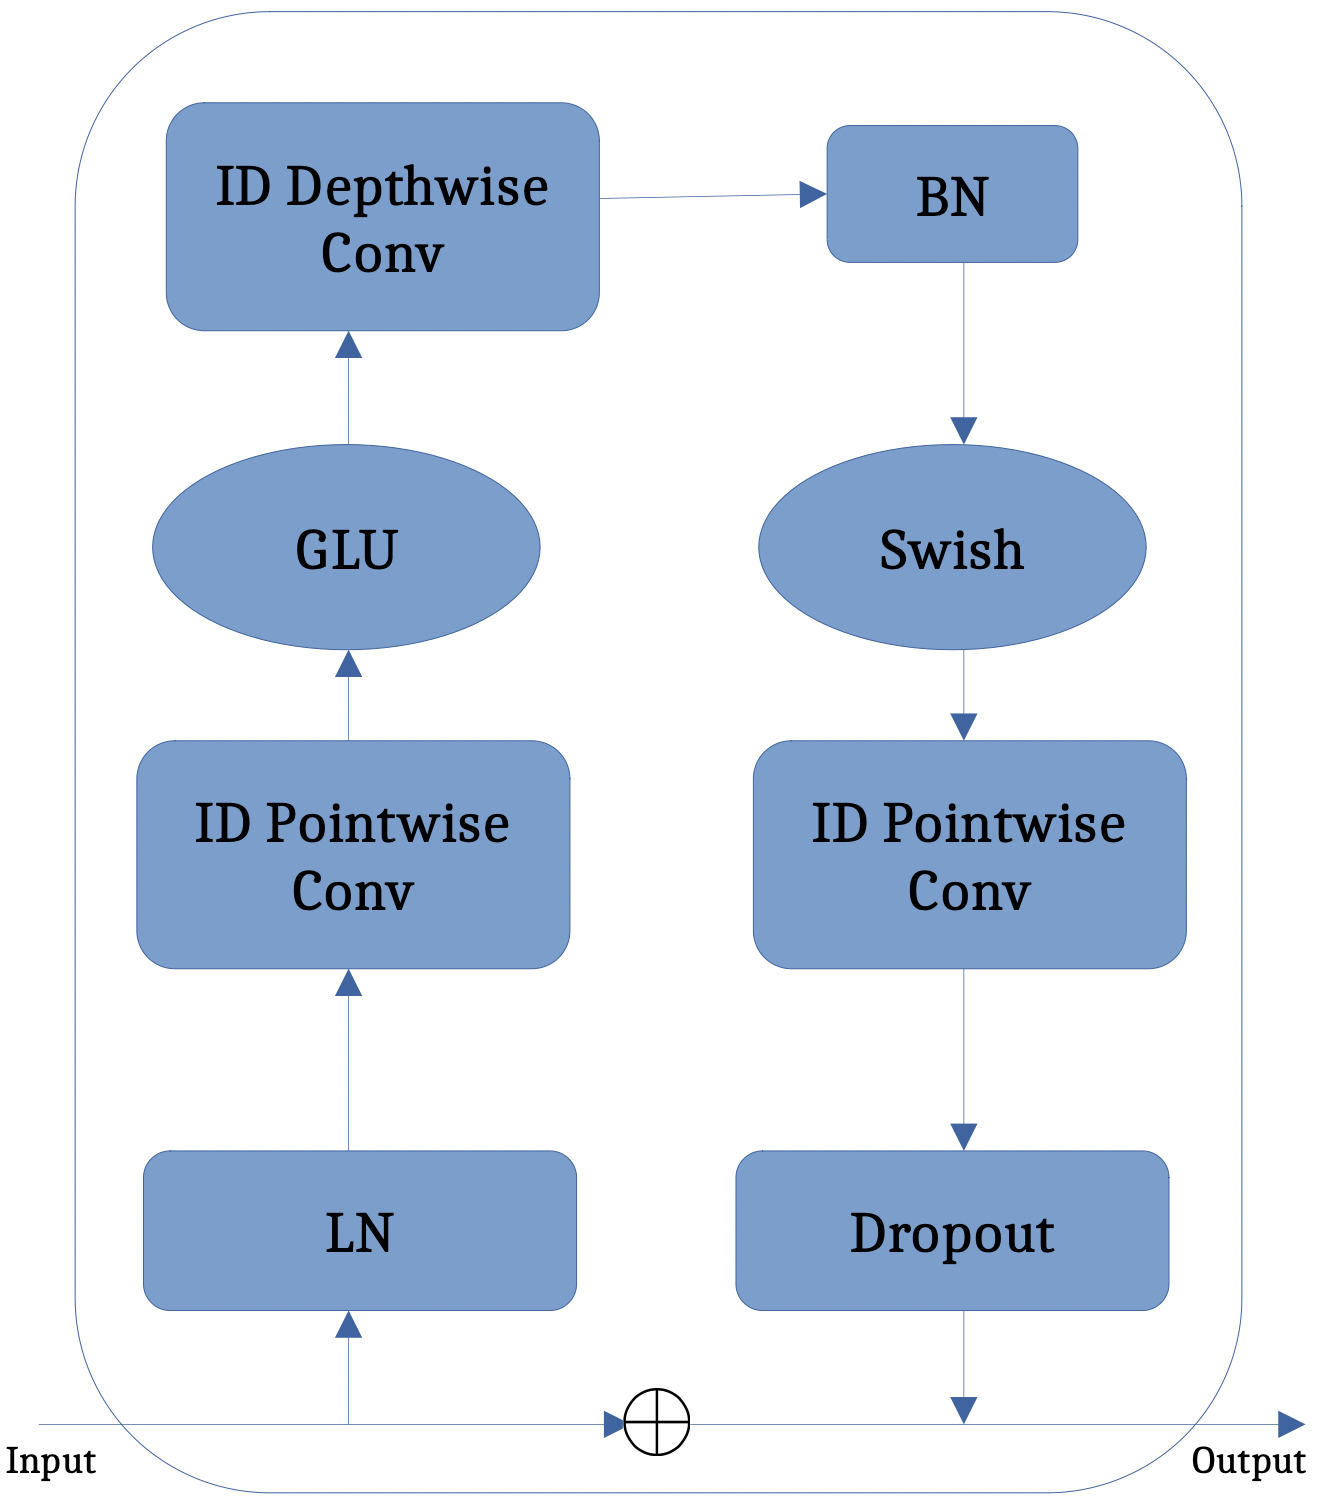
\includegraphics[width=\textwidth]{../images/conv.png}
    \captionof{figure}{Conv Architecture}
    \end{subfigure}
    \begin{subfigure}[b]{0.45\textwidth}
    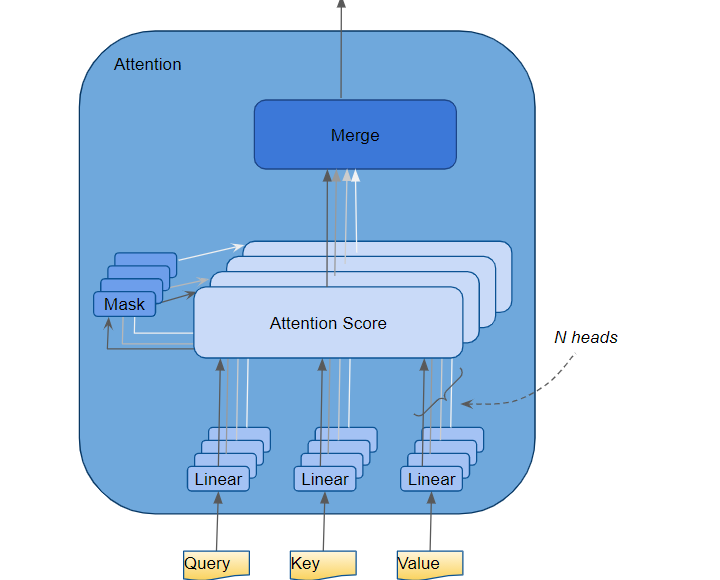
\includegraphics[width=\textwidth]{../images/attention.png}
    \captionof{figure}{Multi-Head Soft Attention}
    \end{subfigure}
    \label{fig:ESPNet}
    \caption{Conformer Building Blocks}
\end{figure}


\begin{figure}
    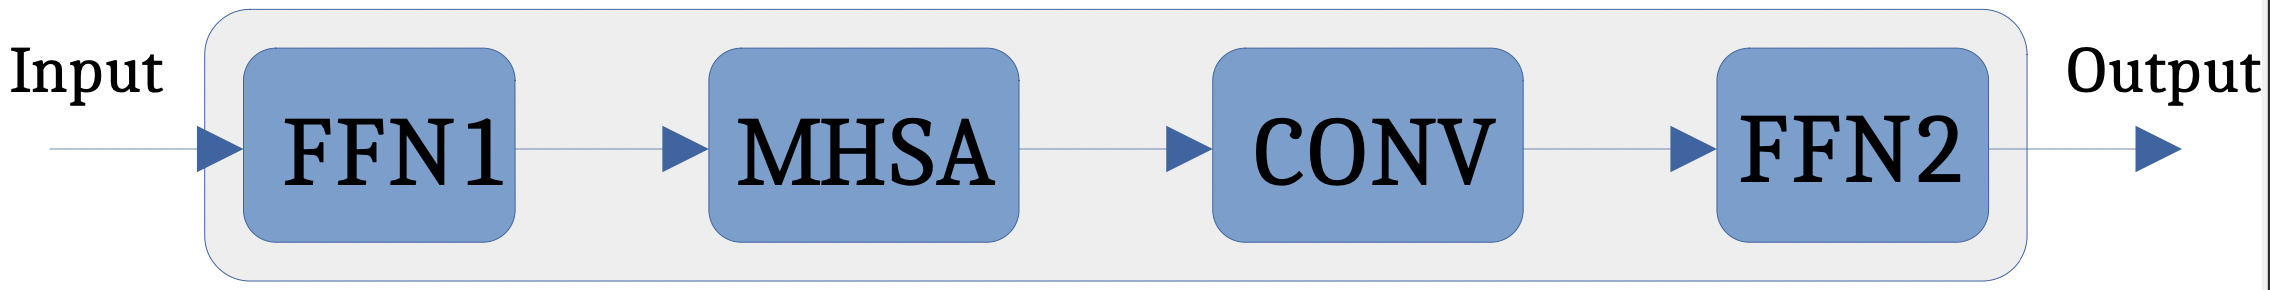
\includegraphics[width=\textwidth]{../images/espnet_pipeline.png}
    \captionof{figure}{Conformer Architecture}
\end{figure}

\newpage

\subsection{Emotion to Speech}
\textbf{Motivation:}

Often the emotion carried out by an utterence cannot be properly conveyed using sign-language.\\
\textbf{Dataset:}

We used RAVDESS \cite{ravdess} dataset to train our model. Since the whole dataset is about 25 GB consisting of about 7356 files. Because of our limited resources, we downloaded about 3000 files and trained our model on it. As a result, the model has accuracy in the range 47-89\% for different emotions.\\
\textbf{Model description:}

The model consists of Conv1D layer, ReLU activation layer,  Dropout layer, Maxpooling 1D layer, Conv1D layer, Dropout layer, Flatten layer, Dense layer, Softmax Activation layer.\\
The optimizer used was an RMSprop optimizer with learning rate = 0.00005, $\rho$ = 0.9
\begin{figure}
\centering
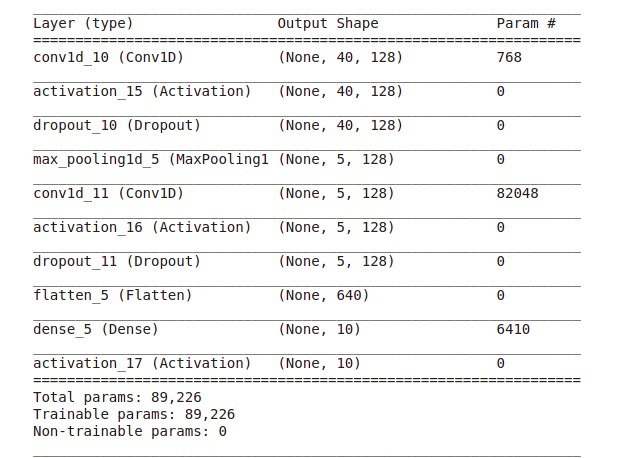
\includegraphics[width=0.8\textwidth]{../images/emo_rec_model.jpeg}
\caption{Emotion Recognition Model Architecture}
\end{figure}
\textbf{Training:}

The input speech signal was converted into 40-dimensional MFCC features and trained on a CNN-based model with a softmax output, trained on Sparse Categorical Cross-Entropy Loss.\\
\textbf{Results:}

The model achieved a test accuracy of 72\% on RAVDESS audio test data consisting of all emotions.

\begin{figure}
    \centering
    \begin{subfigure}[b]{0.3\textwidth}
    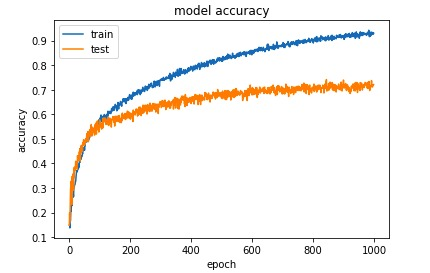
\includegraphics[width=\textwidth]{../images/graph.jpeg}
    \caption{Model accuracy vs epochs}
    \end{subfigure}
    \begin{subfigure}[b]{0.3\textwidth}
    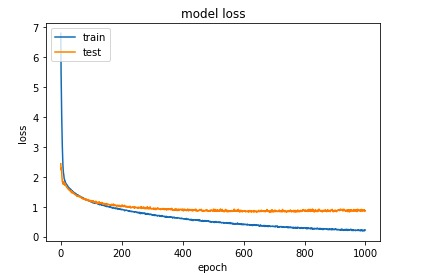
\includegraphics[width=\textwidth]{../images/graph2.jpeg}
    \caption{Train and Validation Loss}
    \end{subfigure}
    \begin{subfigure}[b]{0.3\textwidth}
    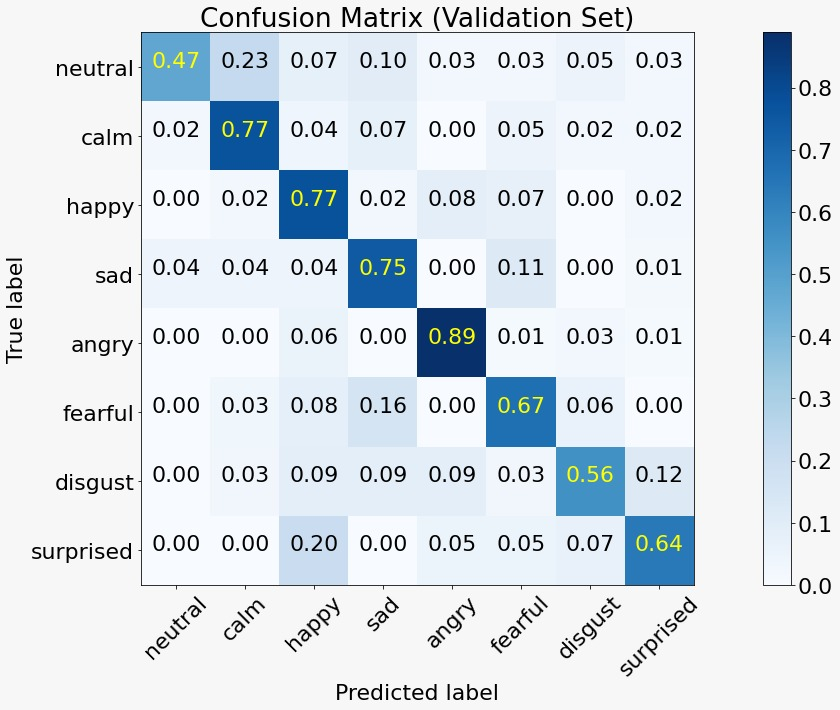
\includegraphics[width=\textwidth]{../images/cm.jpeg}
    \caption{Confusion Matrix}
    \end{subfigure}
    \label{fig:Emotion Recognition}
    \caption{Emotion Recognition Training Stats}
\end{figure}

\subsection{Text to ASL}
So, in order to complete the pipeline, the final step is to convert the decoded text into ASL. But this conversion is not straight forward, because the grammar of ASL is different from Spoken grammar. We tried to find resources that would enable us to complete the pipeline. Most of the resources that we gathered converted each letter of a text to some ASL mapping, but that was not what we intended as it would result in a spelling type output. We also went through some implementations that used Unity or Blender based Avatar Models, to convert text to ASL, but they were limited by their dataset. We came across this \href{https://github.com/arunnair411/Speech-to-ASL}{repository}, which explored this idea in some depth.

It proposed a GAN based interpolation network that used a ASL glossary derived from the decoded English text. The workflow in this repository is as follows:
\begin{itemize}
	\item Translate text to ASL glossary using Transformer model.
	\item Align the ASL Glossary to poses using OpenPose.
	\item Interpolate the poses generated using a Fully-Connected neural network (FCN).
	\item Generate avatar images for each pose using pix2pix GAN and compile as a video.
\end{itemize}
But given the constrained resources, we could not attempt to explore this path. Hence, the final step of the project remains to be completed in the near future.

\section{Web-App for Integration}
We created a Web-App using python's \texttt{streamlit} module, that integrated the different subtasks into one window. THe Web-App contains the facility to record one's own audio, visualize and hear-out the recorded stream and then look into the decoded output from the Speech2Text model as well as the Emotion Recognition model. A demo video for the same is made available \href{https://github.com/soham2109/CS-753-Project/blob/main/presentation/asr_project_demo_video.mkv}{here}.

Here are some snippets that were captured while we were experimenting with the app.
\begin{figure}
    \centering
    \begin{subfigure}[b]{0.3\textwidth}
    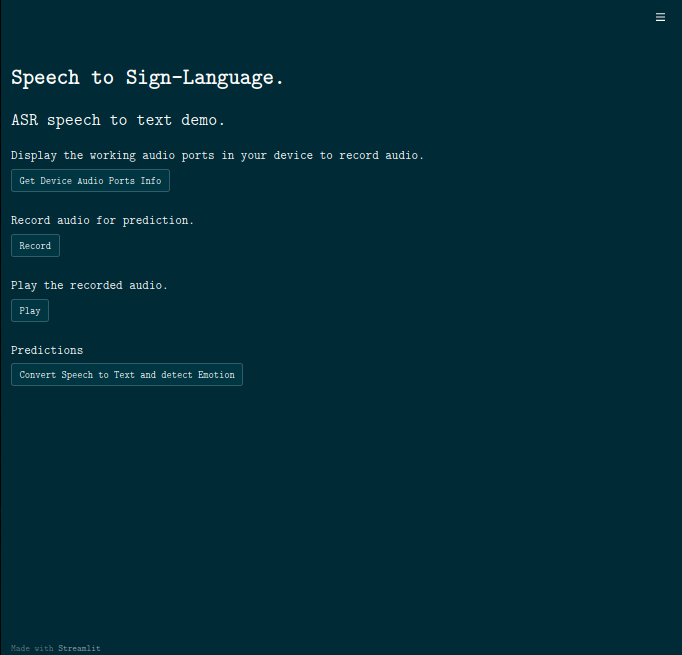
\includegraphics[width=\textwidth]{../images/streamlit_app1.png}
    \caption{Overview of the App}
    \end{subfigure}
    \begin{subfigure}[b]{0.3\textwidth}
    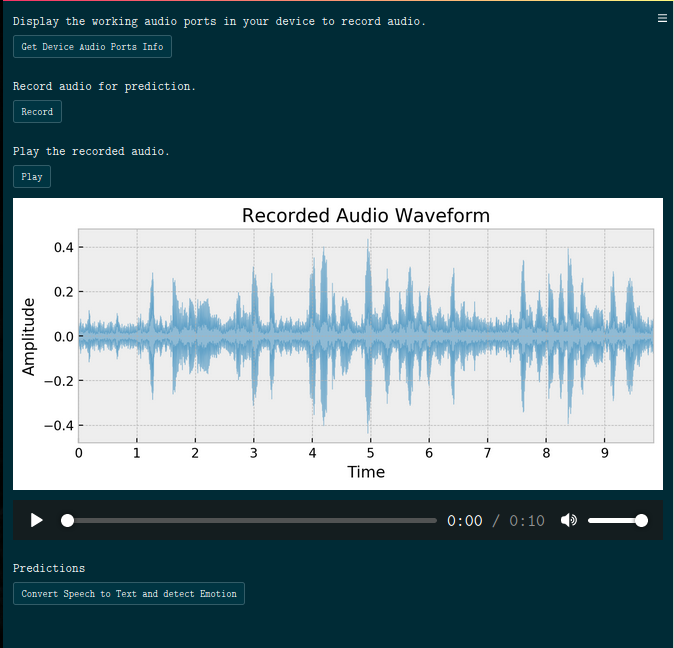
\includegraphics[width=\textwidth]{../images/streamlit_app2.png}
    \caption{Play the recording}
    \end{subfigure}
    \begin{subfigure}[b]{0.35\textwidth}
    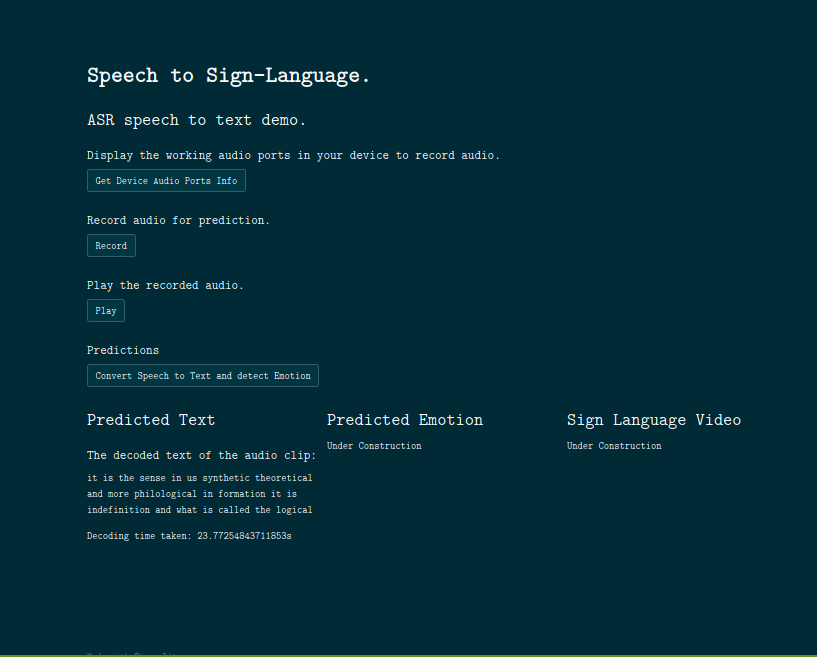
\includegraphics[width=\textwidth]{../images/streamlit_app3.png}
    \caption{Decoded Output}
    \end{subfigure}
    \label{fig:WebApp}
    \caption{WebApp Demo Snippets}
\end{figure}

\section{Work Load Division}
\begin{itemize}
	\item \textbf{Soham Naha}: Speech2Text, WebApp intergration, Presentation
	\item \textbf{Mohit Agarwala}: Presentation, Speech to ASL research
	\item \textbf{Abhinav Goud Bingi}: Speech to Emotion
\end{itemize}

\newpage
\printbibliography %Prints bibliography
\end{document}